\section{Environment Tracking Through Mobile's Camera}
\subsection{Problem Statement}
For the AR application to display navigation labels or arrows, it must correctly detect the environment through the mobile's camera to locate the user's position with respect to the predefined environment, which serves as the basis for placing navigation objects. In addition, changes in positions and angles must also be tracked to ensure that the objects are rendered accurately.

\subsection{Solution}

\subsubsection{Area Targets}
Vuforia Engine provides Area Targets, a powerful environment tracking feature. In Unity, a scanned 3D model of the target environment can be imported as an object of type Area Target, as shown in Figure~\ref{fig:construct-environment-4}. 

After obtaining the scanned 3D model, we import it into Unity as an Area Target. The default Main Camera is then replaced with the Vuforia ARCamera, and we must ensure that Device Tracking is enabled so the system can reliably establish the user’s pose relative to the scanned environment. The imported Area Target appears as a GameObject that includes a preview mesh—this mesh represents the physical space. It serves as the foundation for positioning the navigational labels or arrows. As discussed in Section~\ref{sec:construct-environment}, multiple Area Targets, if appropriately aligned during scanning, can be imported. They will appear at the correct positions relative to each other.

We enable runtime occlusion to improve realism by adding a runtime mesh representation. This process generates a dynamic mesh from the scanned data that acts as an occlusion layer. With the runtime mesh active, virtual objects will be appropriately hidden by physical obstacles (such as walls or furniture), ensuring that the AR content appears naturally embedded in the environment.

\subsubsection{Area Target Observer}\label{subsub:AreaTargetObserver}
Associated with Area Targets is the Area Target Observer, the component that actively manages the tracking of the imported 3D scan. It continuously monitors the pose and status of the Area Target within the scene, providing real-time updates to ensure that navigational labels or arrows remain accurately aligned with the physical environment. The observer retrieves key information—such as the target's bounding box, dimensions, and current tracking state (as shown in Figure~\ref{fig:environment-tracking-1})—which can be used to adjust the placement and orientation of augmented content dynamically.

\begin{figure}[ht]
  \centering
  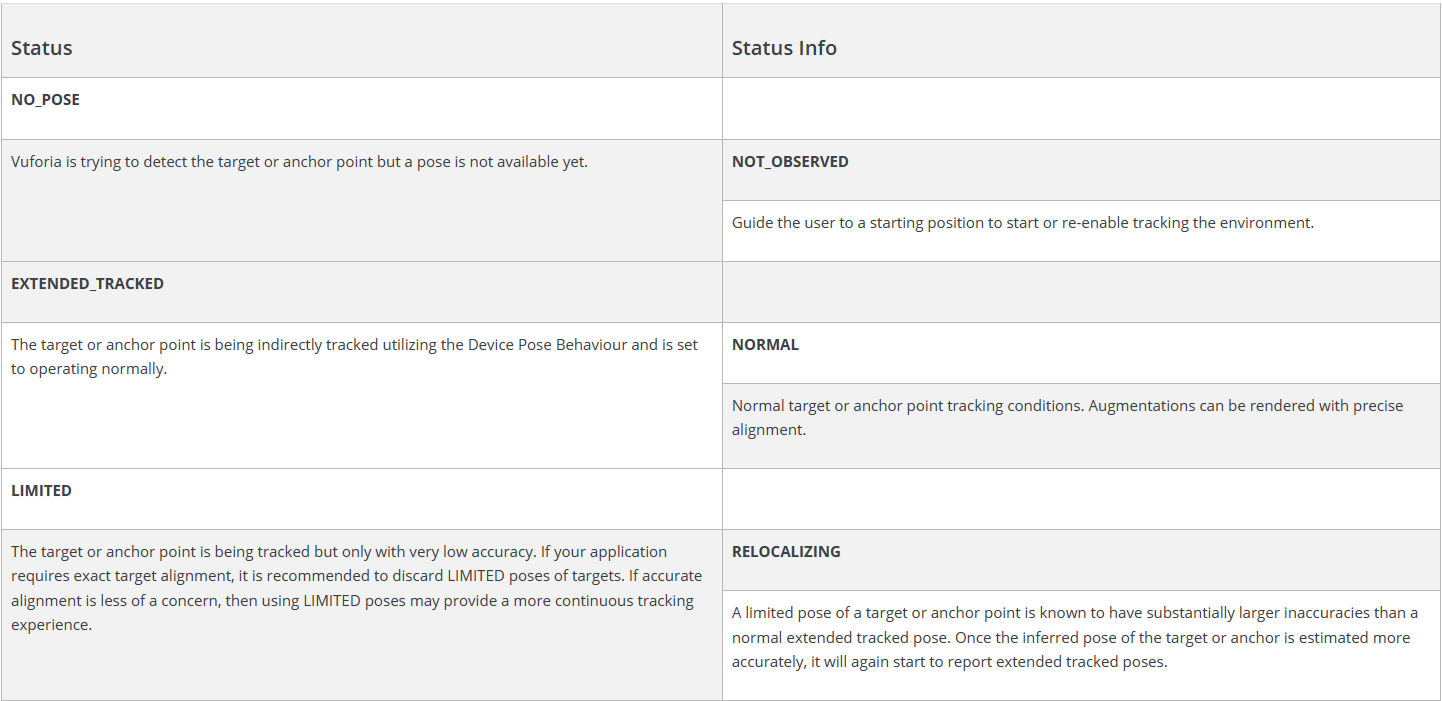
\includegraphics[scale=0.5]{content/resources/images/chap-problems-solutions/environment-tracking-1.PNG}
  \caption{The table listing the available pose status values for Area Targets. \\ \small{Source: \url{https://developer.vuforia.com/library/getting-started/pose-status-and-status-info-unity}}}
  \label{fig:environment-tracking-1}
\end{figure}

Beyond mere tracking, the observer facilitates a richer interaction experience by providing detailed feedback about the environmental context. It continuously assesses the tracking data's reliability, including various states indicating whether a target is fully tracked, partially tracked, or has lost tracking entirely. This detailed status information allows developers to fine-tune the augmented content’s behavior—adjusting its position, orientation, or scale—to adapt to environmental changes and maintain user immersion.

The tracking states of the Area Targets are reported and can be monitored through their Observer Behaviours. The \texttt{ObserverBehaviour} component associated with each Area Target can be retrieved as follows. Note that the Observer can only be retrieved for each Area Target, and it can only be accessed from within the Area Target object.

\begin{lstlisting}[style=cSharp]
ObserverBehaviour mObserverBehaviour = GetComponent<ObserverBehaviour>();
\end{lstlisting}

The current tracking status can be retrieved as follows.

\begin{lstlisting}[style=cSharp]
mObserverBehaviour.OnTargetStatusChanged += OnStatusChanged;
void OnStatusChanged(ObserverBehaviour behaviour, TargetStatus status)
{
    Debug.LogFormat("TargetName: {0}, Status is: {1}, StatusInfo is: {2}", behaviour.TargetName, status.Status, status.StatusInfo);
}
\end{lstlisting}

To further streamline the integration between tracking data and user interface feedback, the system employs global state variables managed through ScriptableObjects. A boolean variable is established for every Area Target to signify whether that particular area is currently being tracked.

\begin{lstlisting}[style=cSharp]
[CreateAssetMenu(fileName = "NewBoolVariable", menuName = "Variables/BoolVariable")]
public class BoolVariable : ScriptableObject
{
    public bool Value;
}
\end{lstlisting}

Whenever there is a change in the tracking status, we update the variables accordingly.

\begin{lstlisting}[style=cSharp]
public BoolVariable isTracked;
void OnStatusChanged(ObserverBehaviour behaviour, TargetStatus status)
{
    if (status.StatusInfo == StatusInfo.NORMAL)
    {
        isTracked.Value = true;
    }
    else
    {
        isTracked.Value = false;
    }
}
\end{lstlisting}

Collecting tracking status data from all monitored areas allows us to create a comprehensive overview of the environment, which is then used to display a clear and informative message to the user regarding their current floor. By aggregating this data, the system determines which specific floor the user is on and updates the interface with a message that confirms this location. This not only reinforces the user’s spatial awareness but also enhances the overall experience by keeping them informed in real time. In cases where none of the defined areas are actively being tracked, the system takes a proactive approach: it issues a warning to the user, advising them to either move towards a known area where tracking is reliable or to re-scan the QR code placed at pre-determined positions throughout the space. This re-scan prompt is designed to quickly recalibrate the tracking system and restore accurate positioning, ensuring users can seamlessly continue their navigation or interaction with the augmented reality content.

\begin{lstlisting}[style=cSharp]
public Text message;
public BoolVariable IsAreaTarget7;
public BoolVariable IsAreaTarget8;
void Update()
{
    if (IsAreaTarget7.Value) {
        message.text = "Tracking 7th floor.";
    }
    else if (IsAreaTarget8.Value) {
        message.text = "Tracking 8th floor.";
    }
    else {
        message.text = "No area target detected. Please move to the area target or re-scan for a position.";
    }
}
\end{lstlisting}

\begin{figure}[ht]
  \centering
  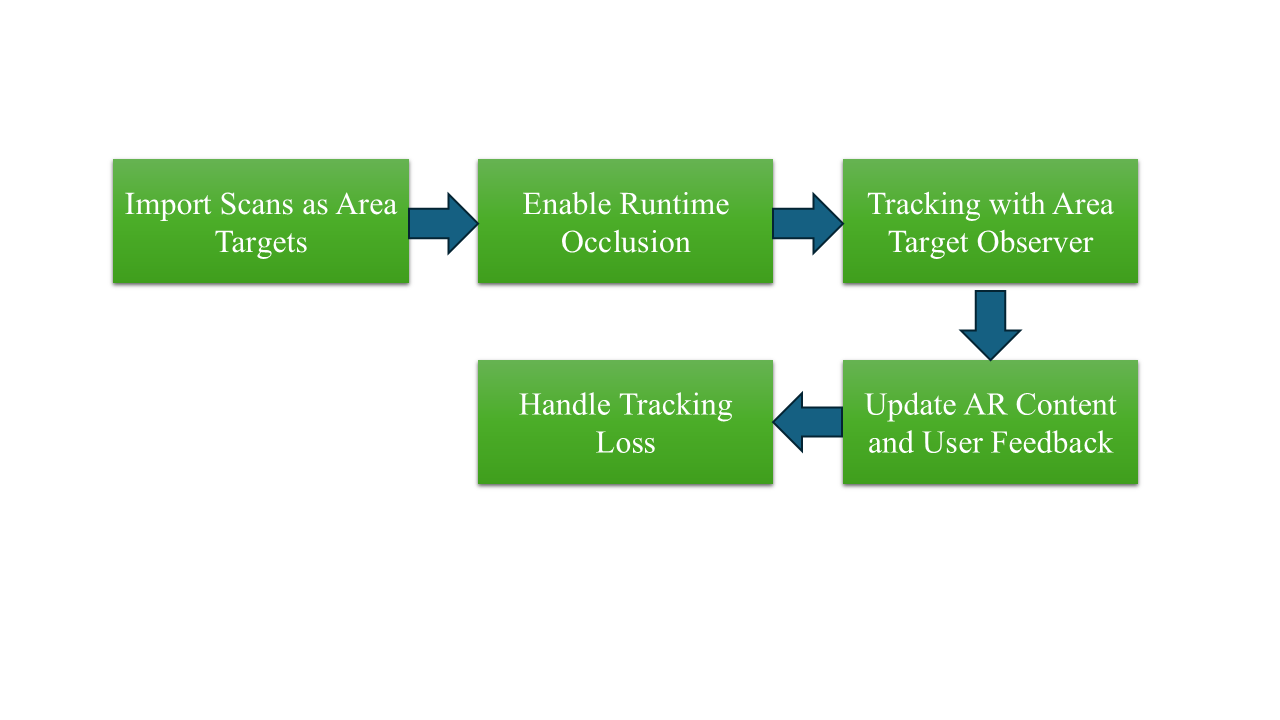
\includegraphics[scale=0.5]{content/resources/images/chap-problems-solutions/environment-tracking-0.PNG}
  \caption{Workflow of Environment Tracking with Area Targets}
  \label{fig:environment-tracking-0}
\end{figure}
